%package list
\documentclass{article}
\usepackage[top=3cm, bottom=3cm, outer=3cm, inner=3cm]{geometry}
\usepackage{graphicx}
\usepackage{url}
%\usepackage{cite}
\usepackage{hyperref}
\usepackage{array}
%\usepackage{multicol}
\newcolumntype{x}[1]{>{\centering\arraybackslash\hspace{0pt}}p{#1}}
\usepackage{natbib}
\usepackage{pdfpages}
\usepackage{multirow}
\usepackage{multirow}
\usepackage[normalem]{ulem}
\useunder{\uline}{\ul}{}



%%%%%%%%%%%%%%%%%%%%%%%%%%%%%%%%%%%%%%%%%%%%%%%%%%%%%%%%%%%%%%%%%%%%%%%%%%%%
%%%%%%%%%%%%%%%%%%%%%%%%%%%%%%%%%%%%%%%%%%%%%%%%%%%%%%%%%%%%%%%%%%%%%%%%%%%%
\newcommand{\csemail}{vmachacaa@ulasalle.edu.pe}
\newcommand{\csdocente}{MSc. Vicente Enrique Machaca Arceda}
\newcommand{\cscurso}{Fundamentos de Lenguajes de
Programación}
\newcommand{\csuniversidad}{Universidad La Salle}
\newcommand{\csescuela}{Escuela Profesional de Ingeniería de Software}
\newcommand{\cspracnr}{05}
\newcommand{\cstema}{Ensamblador}
%%%%%%%%%%%%%%%%%%%%%%%%%%%%%%%%%%%%%%%%%%%%%%%%%%%%%%%%%%%%%%%%%%%%%%%%%%%%
%%%%%%%%%%%%%%%%%%%%%%%%%%%%%%%%%%%%%%%%%%%%%%%%%%%%%%%%%%%%%%%%%%%%%%%%%%%%


\usepackage[english,spanish]{babel}
\usepackage[utf8]{inputenc}
\AtBeginDocument{\selectlanguage{spanish}}
\renewcommand{\figurename}{Figura}
\renewcommand{\refname}{Referencias}
\renewcommand{\tablename}{Tabla} %esto no funciona cuando se usa babel
\AtBeginDocument{%
	\renewcommand\tablename{Tabla}
}

\usepackage{fancyhdr}
\pagestyle{fancy}
\fancyhf{}
\setlength{\headheight}{30pt}
\renewcommand{\headrulewidth}{1pt}
\renewcommand{\footrulewidth}{1pt}
\fancyhead[L]{\raisebox{-0.2\height}{
\includegraphics[width=3cm]{img/logo_salle}}}
\fancyhead[C]{}
\fancyhead[R]{\fontsize{7}{7}\selectfont	\csuniversidad \\ \csescuela \\ \textbf{\cscurso} }
\fancyfoot[L]{MSc. Vicente Machaca}
\fancyfoot[C]{\cscurso}
\fancyfoot[R]{Página \thepage}

\usepackage{listings}
\usepackage{xcolor} % for setting colors

% set the default code style
\lstset{
    frame=tb, % draw a frame at the top and bottom of the code block
    tabsize=4, % tab space width
    showstringspaces=false, % don't mark spaces in strings
    numbers=left, % display line numbers on the left
    commentstyle=\color{green}, % comment color
    keywordstyle=\color{blue}, % keyword color
    stringstyle=\color{red} % string color
}






\begin{document}
%	\nocite{10.5555/1610485}
	\vspace*{10px}
	
	\begin{center}	
		\fontsize{17}{17} \textbf{ Práctica \cspracnr}
	\end{center}
	%\centerline{\textbf{\underline{\Large Título: Informe de revisión del estado del arte}}}
	%\vspace*{0.5cm}
	

	\begin{table}[h]
		\begin{tabular}{|x{4.7cm}|x{4.8cm}|x{4.8cm}|}
			\hline 
			\textbf{DOCENTE} & \textbf{CARRERA}  & \textbf{CURSO}   \\
			\hline 
			\csdocente & \csescuela & \cscurso    \\
			\hline 
		\end{tabular}
	\end{table}	
	
	
	\begin{table}[h]
		\begin{tabular}{|x{4.7cm}|x{4.8cm}|x{4.8cm}|}
			\hline 
			\textbf{PRÁCTICA} & \textbf{TEMA}  & \textbf{DURACIÓN}   \\
			\hline 
			\cspracnr & \cstema & 3 horas   \\
			\hline 
		\end{tabular}
	\end{table}
	
	
	\section{Datos de los estudiantes}
	\begin{itemize}
		\item GIT: \href{https://github.com/Robertohg/FLP}{GIT-Repo}
		\item Integrantes: 
		\begin{itemize}
			\item Roberto Heredia Garland
			
		\end{itemize}		
	\end{itemize}
	
	
	

	
	\section{Ejercicios}\label{sec:ejercicios}
	\begin{enumerate}
		\item Escribir un programa que pida al usuario un número entero y muestre por pantalla si es par o impar.
	

	
		\begin{lstlisting}[language={[x86masm]Assembler}, basicstyle=\small]
.data 
num:.asciiz  "Ingrese un numero:\n"
even: .asciiz "El numero  es par "
oddr:.asciiz  "El numero es impar "

.text  

main:
addi $t0, $0, 2 
la $a0, num  
li $2, 4
syscall

li $2, 5
syscall

div $2, $t0 
mfhi $t1
beq $t1, $0, print_1  
la $a0, odd  
li $2, 4
syscall

j fin
print_1: la $a0, even
li $2, 4
syscall

j fin
fin: li $2, 10
syscall

	jr	$ra

	
		   \end{lstlisting}
	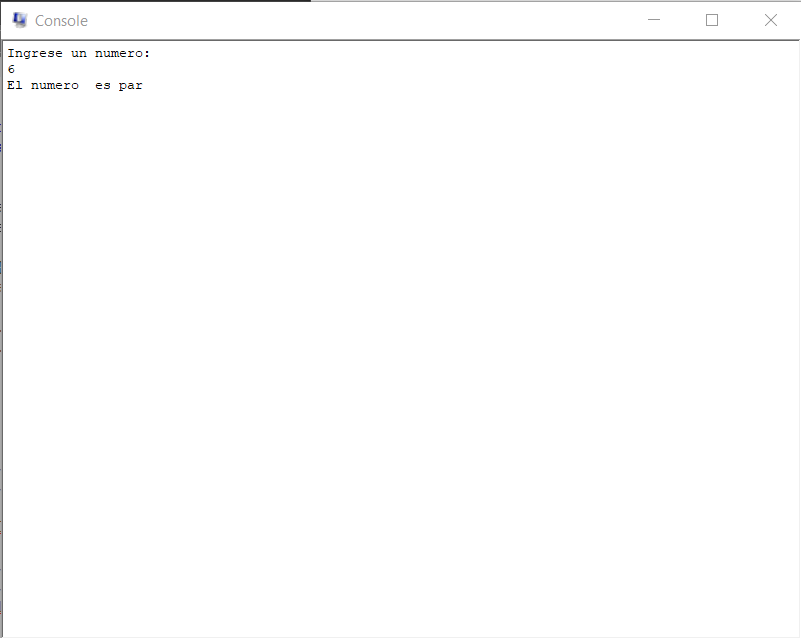
\includegraphics[width=8cm]{img/eje1.png}
	\newpage
	\item Escribir un programa que pida al usuario un número entero positivo y muestre por pantalla todos los números impares desde 1 hasta ese número.
	
		\begin{lstlisting}[language={[x86masm]Assembler}, basicstyle=\small]
.data 	
 num:.asciiz  "Ingrese un numero: \n"
 odds: .asciiz "\nLos numeros impares hasta "
 num1: .asciiz " son: "
.text 
main:
	li $v0, 4
	la $a0, num 
	syscall 

	li $v0, 5
	syscall
	move $t0, $v0
	
	li $v0, 4
	la $a0, odds 
	syscall	

	li $v0, 1
	move $a0, $t0
	syscall

	li $v0, 4
	la $a0, num1   
	syscall

	li $t1, 1
	loop1:
		bge $t1, $t0 end_loop1 
		
		li $v0, 1
		move $a0, $t1 
		syscall 

		li $a0, 32 
		li $v0, 11 
		syscall
		
		add $t1, $t1, 2
		j loop1

        end_loop1:
                li $v0, 10
                syscall
                
		   \end{lstlisting}	
	
	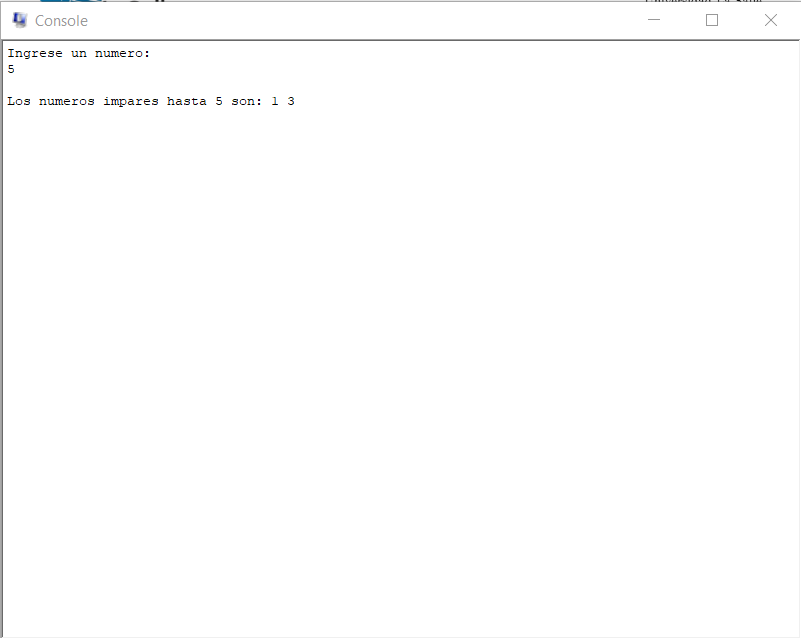
\includegraphics[width=8cm]{img/eje2.png}
		\newpage
		
	\item Escribir un programa que pida al usuario un número entero y muestre por pantalla si es un número primo o no.
	
		\begin{lstlisting}[language={[x86masm]Assembler}, basicstyle=\small]

.data
num: .asciiz "\n Ingrese un numero: "
noprimo: .asciiz "\n El numero no es primo"
primo: .asciiz "\n El numero es primo"

.text

main:	
    li $v0, 4
	la $a0, num  
	syscall
	li $v0, 5 
	syscall
	move $t0, $v0 
	li $t1, 2
	
loop1:   
        beq $t0, $t1 si_primo   
	div $t0, $t1  
	mfhi $t2  
	beqz $t2, no_primo  
	addi $t1, $t1 1
	j loop1
	
no_primo:
	li $v0, 4
	la $a0, noprimo   
	syscall
	j exit
	
si_primo:
	li $v0, 4
	la $a0, primo 
	syscall
	j exit
	
exit:	li $v0, 10 
	syscall
		   \end{lstlisting}	
	
	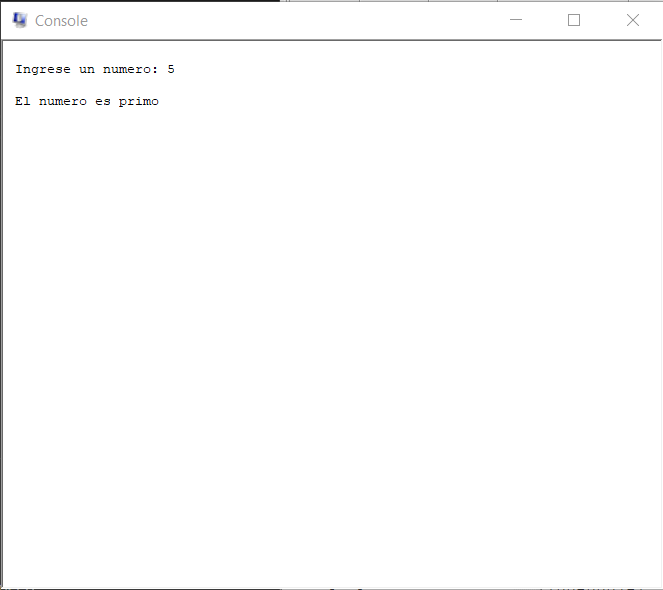
\includegraphics[width=8cm]{img/eje3.png}
	
	\clearpage
	%\bibliographystyle{apalike}
	%\bibliographystyle{IEEEtranN}
	%\bibliography{bibliography}
		\end{enumerate}
	
\end{document}